\chapter{Planificación}\label{ch:planificacion}
%************************************************

\section{Planificación inicial}
La planificación mostrada a continuación fue realizada al inicio del proyecto, siendo ésta de muy alto nivel. De momento no vamos a indagar en detalles específicos sobre las metodologías usadas o la planificación real, esto en cambio, se detallará en la sección posterior.

\vspace{0.3cm}

Un trabajo de fin de grado está compuesto por 12 créditos en el Título de Grado en Ingeniería Informática de la Universidad de Granada. Además, por normativa de la universidad ea cada crédito ECTS se le establece un número de 25 horas de trabajo. En total, 300 horas de trabajo. Esto se traduce a casi dos meses de trabajo si contamos con una jornada laboral completa y descanso los fines de semana.

\vspace{0.3cm}

Aunque, al fin y al cabo, sigue siendo una estimación muy ligera a lo que realmente terminará siendo. Por lo que la estimación que usaré a continuación será en base a las fechas del inicio y el fin de la elaboración del proyecto, en mi caso será desde inicios de Julio hasta finales de Octubre:

\vspace{0.3cm}

\begin{figure}[bth]

    \myfloatalign
    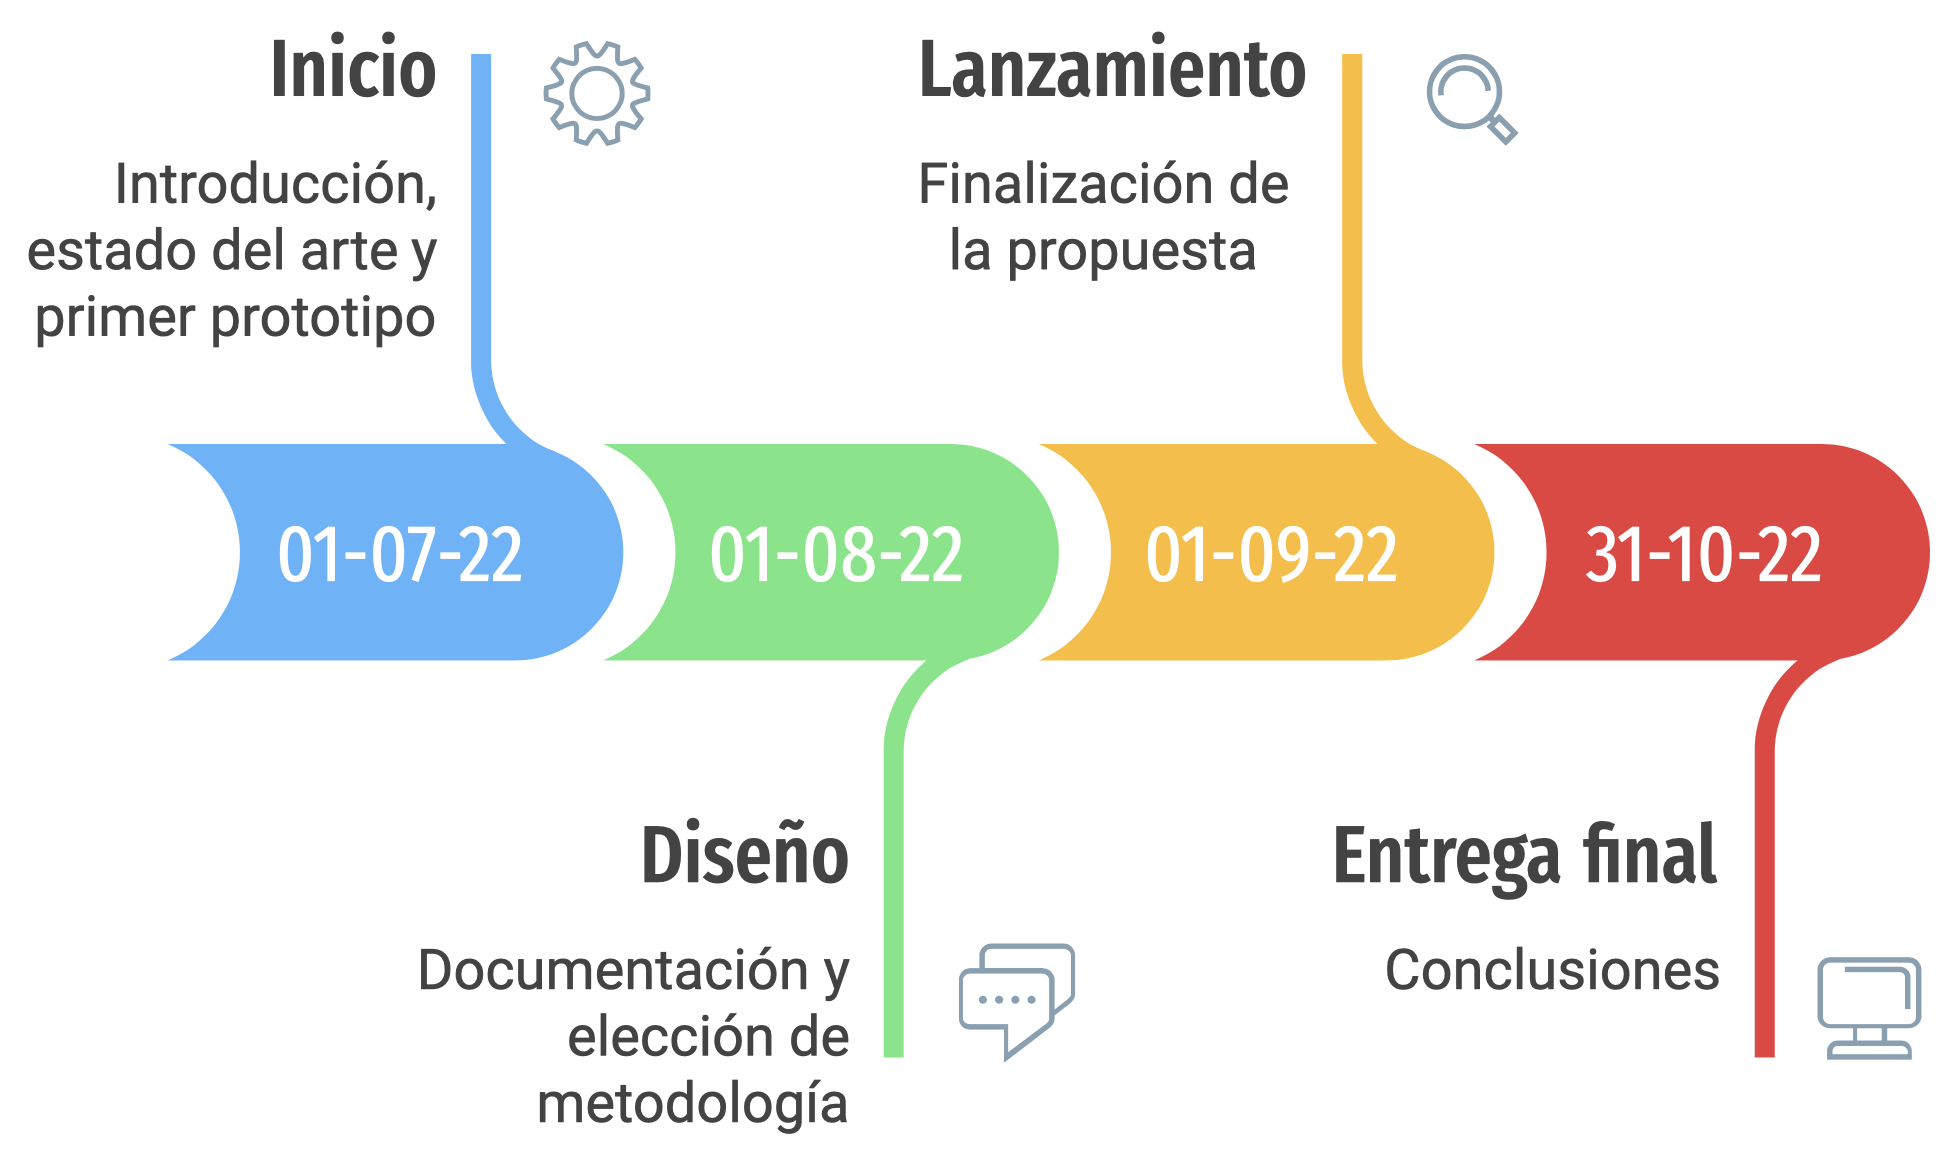
\includegraphics[width=0.9\textwidth]{gfx/plan-simple.png}
    \caption[Planificación inicial del proyecto]{Visión general sobre la estructura de la elaboración del proyecto.}\label{gfx:plan-simple}

\end{figure}

\newpage

\begin{itemize}
    \item Inicio \textit{(01-07-22 $\sim$ 01-08-22)}: etapa de planificación de la memoria y el estado del arte. Además se intentará tener un primer prototipo de la aplicación.
    \item Diseño \textit{(01-08-22 $\sim$ 01-09-22)}: inicios de la codificación y la elaboración de la parte correspondiente de la memoria.
    \item Lanzamiento \textit{(01-09-22 $\sim$ 01-10-22)}: etapa donde se realizarán pruebas de usuario y finalizará la codificación.
    \item Entrega final \textit{(01-10-22 $\sim$ 31-10-22)}: elaboración de conclusiones respecto al cumplimiento del software y sus posibles mejoras.
\end{itemize}

\section{Planificación detallada}\label{ch:planificacion_detallada}

Al planificar el proyecto de la manera que está representado en la figura \ref{gfx:plan-simple}, he optado por una metodología ágil para confrontar el proyecto.

\vspace{0.3cm}

Esto es debido a que necesitamos un marco de trabajo que sea adaptativo y flexible a la hora de realizar distintas pruebas y su correspondiente arreglo a la hora de encontrarnos errores o cambios exigidos por el cliente.

\vspace{0.3cm}

Todas estas ventajas son las que me encaminado a elegir esta metodología, la cual parece tener las mejores prácticas para este proyecto en concreto.

\vspace{0.3cm}

Hoy en día, el marco de trabajo más ampliamente conocido y a la vez el más ventajoso sea posiblemente SCRUM. Se ha elegido este marco de trabajo para tener el mejor resultado posible a la hora de abarcar el proyecto. Sus principales ventajas son la flexibilidad y la productividad, pero abarcaremos más en detalle sus propiedades en la sección \ref{sec:metodologia}.

\vspace{0.3cm}

En la siguiente página se podrá ver la planificación en mucho mayor detalle. En la tabla (figura \ref{gfx:plan-detallado}) se detalla toda la perspectiva del trabajo, desde las partes más fundamentales de la documentación hasta el diseño de la propia aplicación.

\begin{figure}[hbtp]

    \myfloatalign
    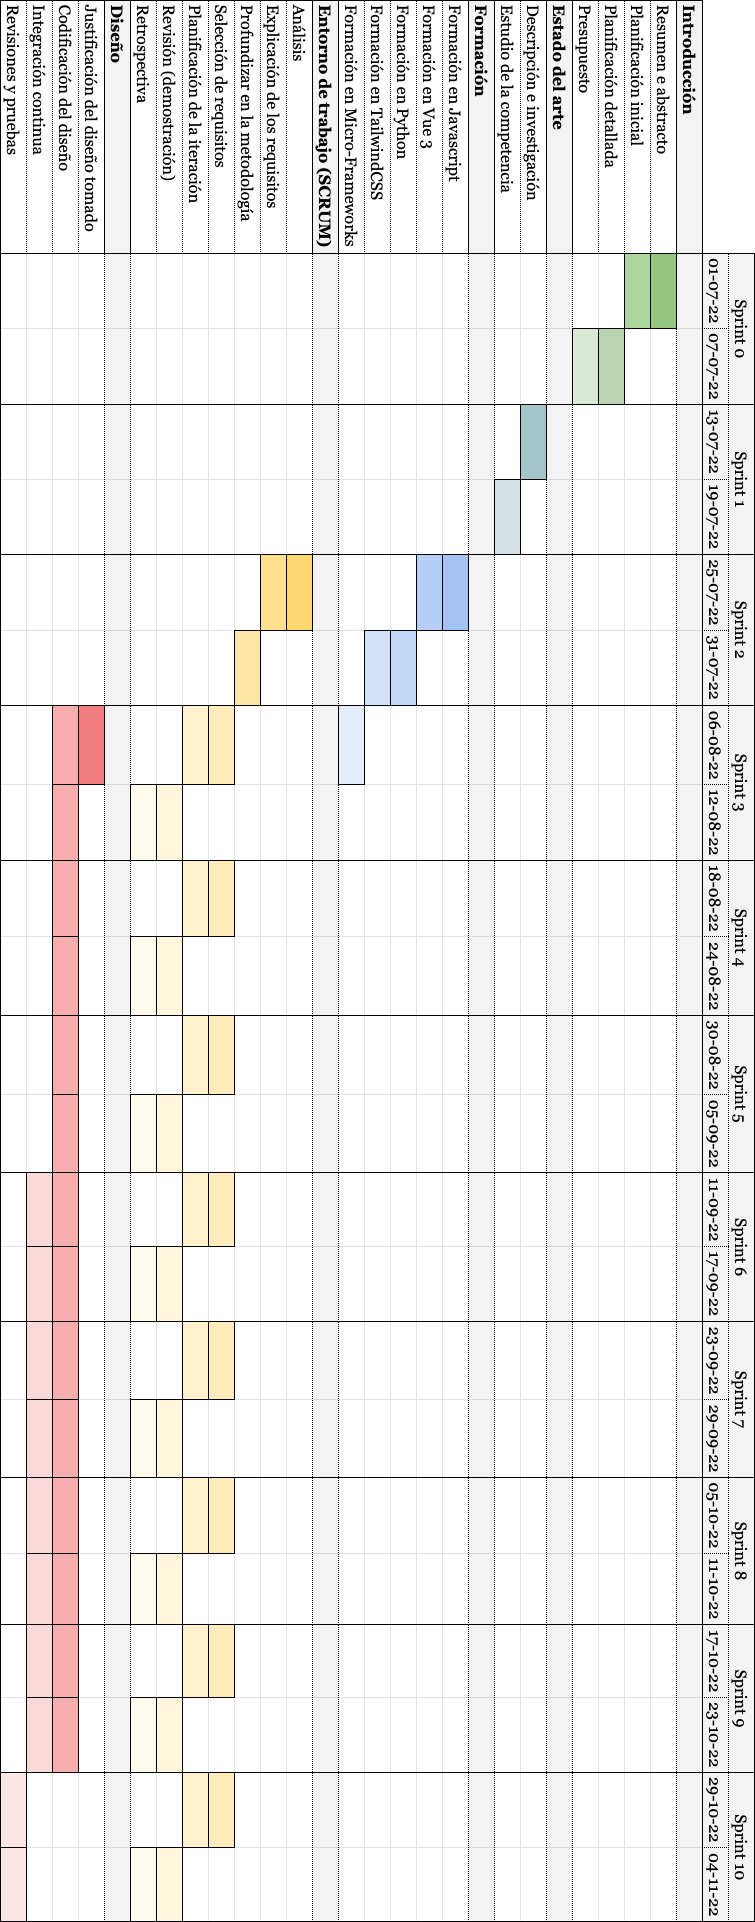
\includegraphics[width=0.73\textwidth]{gfx/plan-detallado.png}
    \caption[Planificación detallada del proyecto]{Visión más detallada sobre la estructura de la elaboración del proyecto.}\label{gfx:plan-detallado}

\end{figure}

\newpage

\section{Presupuesto}

Las horas de trabajo las tenemos especificadas desde un principio, es decir, el trabajo de fin de grado por normativa tiene 300 horas. Gracias a las páginas web como Talent podemos saber que el salario medio de un desarrollador web está en torno de los 11,79 €. \cite{Salario-Desarrollador-Web} En cuanto a las horas de trabajo y sus diferentes secciones quedaría de la siguiente manera.

\vspace{0.3cm}

\begin{table}[h]

    \centering
    \setlength\arrayrulewidth{0.8pt}

    \begin{tabular}{ >{\centering\arraybackslash}m{1.2in} | >{\centering\arraybackslash}m{0.8in} | >{\centering\arraybackslash}m{0.8in} | >{\centering\arraybackslash}m{0.8in} |}

\cline{2-4}
                                                                          & \cellcolor{RoyalBlue}{Horas} & \cellcolor{RoyalBlue}{Porcentaje} & \cellcolor{RoyalBlue}{Coste} \\ \hline
\multicolumn{1}{|c|}{\cellcolor{RoyalBlue}\textbf{Introducción}}       & $16.9014$                                              & $5.6338$ \%                                                 & $199.27$ €                                             \\ \hline
\multicolumn{1}{|c|}{\cellcolor{RoyalBlue}\textbf{Estado del arte}}    & $8.4507$                                               & $2.8169$ \%                                                 & $99.64$ €                                              \\ \hline
\multicolumn{1}{|c|}{\cellcolor{RoyalBlue}\textbf{Formación}}          & $21.1267$                                              & $7.0422$ \%                                                 & $249.08$ €                                             \\ \hline
\multicolumn{1}{|c|}{\cellcolor{RoyalBlue}\textbf{Entorno de trabajo}} & $147.8873$                                             & $49.2957$ \%                                                & $1743.59$ €                                            \\ \hline
\multicolumn{1}{|c|}{\cellcolor{RoyalBlue}\textbf{Diseño}}             & $105.6338$                                             & $35.2112$ \%                                                & $1245.42$ €                                            \\ \hline
\multicolumn{1}{|c|}{\cellcolor{RoyalBlue}\textbf{Total}}              & $\approx$ $300$                                                & $\approx$ $100$ \%                                                  & $3536.99$ €                                            \\ \hline
\end{tabular}

    \caption[Presupuesto de la mano de obra]{Presupuesto de la mano de obra, junto con las horas trabajadas.}\label{table:presupuesto-obra-de-mano}

\end{table}

En base a ello, podemos calcular que unas 300 horas de trabajo equivaldrían a 3537 € y la elaboración de la documentación o el manual equivaldrían a 300 €. En total 3837 € solamente por la mano de obra.

\vspace{0.3cm}

Buscaré además el uso de herramientas gratuitas de diferentes servicios para el mantenimiento del servicio web. En los servicios como Heroku varían los precios entre 100 € y 200 € al mes, pero también poseen herramientas gratuitas y muy limitadas, lo que nos permitirá un gran ahorro al inicio del proyecto. Igualmente para el proyecto necesitaré un área de trabajo y un ordenador capaz de manejar dicho proyecto.

\vspace{0.3cm}

\begin{table}[h]

    \centering
    \setlength\arrayrulewidth{0.8pt}

    \begin{tabular}{ >{\centering\arraybackslash}m{1.2in} | >{\centering\arraybackslash}m{0.8in} | >{\centering\arraybackslash}m{0.8in} |}

    \cline{2-3}
                                                                              & \cellcolor{RoyalBlue}{Cantidad} & \cellcolor{RoyalBlue}{Coste} \\ \hline
    \multicolumn{1}{|c|}{\cellcolor{RoyalBlue}\textbf{Espacio de trabajo}} & $4$ meses                                                 & $\approx$ $400$ €                                                \\ \hline
    \multicolumn{1}{|c|}{\cellcolor{RoyalBlue}\textbf{Ordenador}}          & $1$                                                       & $\approx$ $900$ €                                                \\ \hline
    \multicolumn{1}{|c|}{\cellcolor{RoyalBlue}\textbf{Total}}              &                                                         & $\approx$ $1300$ €                                               \\ \hline
    \end{tabular}

    \caption[Presupuesto de servicios adicionales]{Presupuesto de servicios adicionales, junto con las diferentes cantidades.}\label{table:presupuesto-adicional}

\end{table}

De modo, que el coste total del proyecto sería la suma de ambas cantidades. En este caso, quedaría en 5137 €.